\chapter{Introduction}\label{chap:intro}
\section{Von Neumann Architecture and the Memory Wall}\label{sec:memwall}
The field of computing is at a critical point. For decades, the industry has relied on the von Neumann architecture, 
which physically separates processing and memory units. 
While incredibly successful, this paradigm has created an inherent "memory wall" \cite{gholami_ai_2024}, where the time and energy spent moving 
data between the CPU and memory now dominate the cost of computation. 
This bottleneck is especially highlighted in data-intensive fields like artificial intelligence and machine learning, 
domains heavily reliant on massive parallel operations such as Matrix-Vector Multiplication (MVM) and Matrix-Matrix Multiplication (MM) \cite{gholami_ai_2024,khan_landscape_2024}. 
As Moore's Law slows, only shrinking transistors is no longer a viable path to performance gains, creating the need for new computing architectures.

\section{Dissertation Objective and Motivation}\label{sec:obj}

The "memory wall" has motivated a global research effort into new, beyond von Neumann, computing paradigms. 
Among the most promising is Computing Near-Memory (CNM) and Computing In-Memory (CIM) \picref{fig:cim}, which idea is to perform computation directly where data is stored, eliminating the costly data movement \cite{khan_landscape_2024}.
Among the CIM branches, Phase-Change Memory (PCM) has emerged as a possible candidate to enable Analog In-Memory Computing (AIMC) as its analog resistance states can naturally 
represent the weights of a neural network and the way the crossbar is configured allows for efficient analog and parallel computation.

However, designing and fabricating new hardware accelerators is a high-risk, high-capital process. 
Before committing to silicon, it is essential to have robust virtual platforms to explore architectural trade-offs, 
validate functionality, and co-design the necessary software. This project is motivated by the need for such virtual prototype.

The primary objective of this dissertation is to implement, and validate a virtual prototype of a PCM-based AIMC accelerator within the GVSoC \cite{bruschi_gvsoc_2021} simulator for the PULP platform.

To achieve this objective two main goals were established:\\
Develop a C++ model of a PCM accelerator capable of performing MVM operations, integrated as a memory-mapped peripheral in GVSoC.\\
Investigate and implement performance optimisations for the simulation model itself to allow for efficient and fast simulation even on limited hardware resources.

\begin{figure}[H]
  \centering
  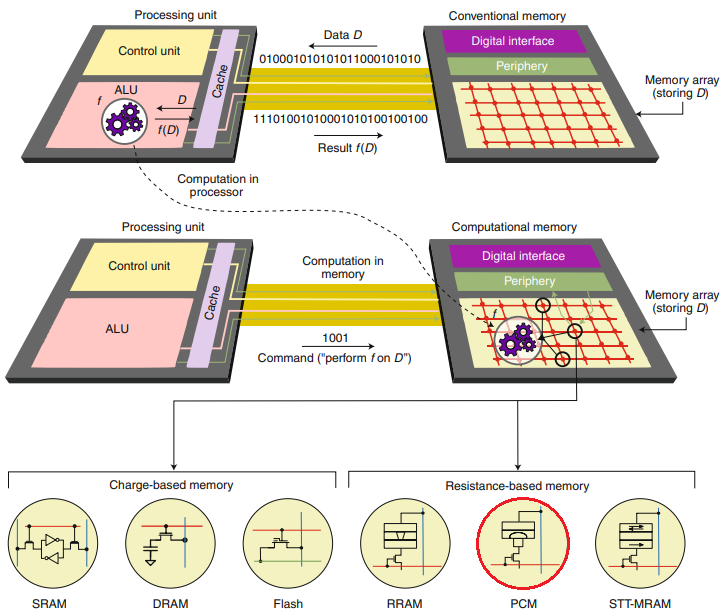
\includegraphics[width=0.8\textwidth]{Figures/CIM.png}
  \caption{Computing In-Memory (CIM) architecture overview, moving computation closer to memory to alleviate the von Neumann bottleneck. Adapted from \cite{sebastian_memory_2020}.}
  \label{fig:cim}
\end{figure}

\section{Summary of Contributions}\label{sec:contri}
This dissertation makes several contributions to the field of hardware acceleration and virtual prototyping for next-generation computing architectures. 
The primary outcomes of this research are the following:\\
A configurable virtual prototype of a PCM accelerator. 
The core contribution is a fully functional C++ model of a PCM-based AIMC accelerator integrated into the GVSoC framework. 
This model is not just a theoretical construct but a working, configurable, peripheral that can be simulated within a complete System-on-Chip 
environment, serving as a valuable tool for architectural exploration.\\

Demonstration and analysis of simulation optimisation techniques. 
This work demonstrates the effectiveness of applying advanced software optimisation principles to the task of hardware simulation. 
By implementing and benchmarking techniques such as flattened data buffers and multithreading, this project provides concrete data 
on how to significantly improve the performance and scalability of virtual prototyping, making large-scale experiments more feasible even on limited computational resources.

